% **************************************************
% Document Class Definition
% **************************************************
\documentclass[%
	paper=A4,					% paper size --> A4 is default in Germany
	twoside=true,				% onesite or twoside printing
	openright,					% doublepage cleaning ends up right side
	parskip=full,				% spacing value / method for paragraphs
	chapterprefix=true,			% prefix for chapter marks
	11pt,						% font size
	headings=normal,			% size of headings
	bibliography=totoc,			% include bib in toc
	listof=totoc,				% include listof entries in toc
	titlepage=on,				% own page for each title page
	captions=tableabove,		% display table captions above the float env
	draft=false,				% value for draft version
]{scrreprt}%

% **************************************************
% Debug LaTeX Information
% **************************************************
%\listfiles

% **************************************************
% Information and Commands for Reuse
% **************************************************
\newcommand{\thesisTitle}{Neural Style}
\newcommand{\thesisName}{Alejandro Avil\'es}
\newcommand{\thesisSubject}{Hierarchical Convolutional Neural Networks}
\newcommand{\thesisDate}{April 25, 2016}
\newcommand{\thesisVersion}{My First Draft}

\newcommand{\thesisFirstReviewer}{Fernando Berzal}
\newcommand{\thesisFirstReviewerUniversity}{\protect{University of Granada}}
\newcommand{\thesisFirstReviewerDepartment}{Intelligent Databases and Information System}

\newcommand{\thesisSecondReviewer}{John Doe}
\newcommand{\thesisSecondReviewerUniversity}{\protect{Clean Thesis Style University}}
\newcommand{\thesisSecondReviewerDepartment}{Department of Clean Thesis Style}

\newcommand{\thesisFirstSupervisor}{Jane Doe}
\newcommand{\thesisSecondSupervisor}{John Smith}

\newcommand{\thesisUniversity}{\protect{Clean Thesis Style University}}
\newcommand{\thesisUniversityDepartment}{Department of Clean Thesis Style}
\newcommand{\thesisUniversityInstitute}{Institut for Clean Thesis Dev}
\newcommand{\thesisUniversityGroup}{Clean Thesis Group (CTG)}
\newcommand{\thesisUniversityCity}{City}
\newcommand{\thesisUniversityStreetAddress}{Street address}
\newcommand{\thesisUniversityPostalCode}{Postal Code}

% **************************************************
% Load and Configure Packages
% **************************************************
\usepackage[utf8]{inputenc}		% defines file's character encoding
\usepackage[english]{babel} % babel system, adjust the language of the content
\usepackage[					% clean thesis style
	figuresep=colon,%
	sansserif=false,%
	hangfigurecaption=false,%
	hangsection=true,%
	hangsubsection=true,%
	colorize=full,%
	colortheme=bluemagenta,%
	bibsys=bibtex,%
	bibfile=bib-refs,%
	bibstyle=alphabetic,%
]{cleanthesis}

\hypersetup{					% setup the hyperref-package options
	pdftitle={\thesisTitle},	% 	- title (PDF meta)
	pdfsubject={\thesisSubject},% 	- subject (PDF meta)
	pdfauthor={\thesisName},	% 	- author (PDF meta)
	plainpages=false,			% 	-
	colorlinks=false,			% 	- colorize links?
	pdfborder={0 0 0},			% 	-
	breaklinks=true,			% 	- allow line break inside links
	bookmarksnumbered=true,		%
	bookmarksopen=true			%
}

% **************************************************
% Document CONTENT
% **************************************************
\begin{document}

% --------------------------
% rename document parts
% --------------------------
%\renewcaptionname{ngerman}{\figurename}{Abb.}
%\renewcaptionname{ngerman}{\tablename}{Tab.}
\renewcaptionname{english}{\figurename}{Fig.}
\renewcaptionname{english}{\tablename}{Tab.}

% --------------------------
% Front matter
% --------------------------
\pagenumbering{roman}			% roman page numbing (invisible for empty page style)
\pagestyle{empty}				% no header or footers
% !TEX root = ../thesis.tex
%
% ------------------------------------  --> cover title page
\begin{titlepage}
	\pdfbookmark[0]{Cover}{Cover}
	\flushright
	\hfill
	\vfill
	{\LARGE\thesisTitle \par}
	\rule[5pt]{\textwidth}{.4pt} \par
	{\Large\thesisName}
	\vfill
	\textit{\large\thesisDate} \\
	Version: \thesisVersion
\end{titlepage}


% ------------------------------------  --> main title page
\begin{titlepage}
	\pdfbookmark[0]{Titlepage}{Titlepage}
	\tgherosfont
	\centering

	
\includegraphics[width=5cm]{gfx/logo.png} \\[4mm]
	{\Large \thesisUniversity} \\[4mm]
	\textsf{\thesisUniversityInstitute} \\
	\textsf{\thesisUniversityDepartment} \\
	\textsf{\thesisUniversityGroup} \\

	\vfill
	{\large \thesisSubject} \\[5mm]
	{\LARGE \color{ctcolortitle}\textbf{\thesisTitle} \\[10mm]}
	{\Large \thesisName} \\[5mm]

	\vfill
	% \begin{minipage}[t]{.27\textwidth}
	% 	\raggedleft
	% 	\textit{1. Reviewer}
	% \end{minipage}
	% \hspace*{15pt}
	% \begin{minipage}[t]{.65\textwidth}
	% 	{\Large \thesisFirstReviewer} \\
	%   	{\small \thesisFirstReviewerDepartment} \\[-1mm]
	% 	{\small \thesisFirstReviewerUniversity}
	% \end{minipage} \\[5mm]
	% \begin{minipage}[t]{.27\textwidth}
	% 	\raggedleft
	% 	\textit{2. Reviewer}
	% \end{minipage}
	% \hspace*{15pt}
	% \begin{minipage}[t]{.65\textwidth}
	% 	{\Large \thesisSecondReviewer} \\
	%   	{\small \thesisSecondReviewerDepartment} \\[-1mm]
	% 	{\small \thesisSecondReviewerUniversity}
	% \end{minipage} \\[10mm]
	% \begin{minipage}[t]{.27\textwidth}
	% 	\raggedleft
	% 	\textit{Supervisor}
	% \end{minipage}
	% \hspace*{15pt}
	% \begin{minipage}[t]{.65\textwidth}
	% 	\thesisFirstSupervisor\
	% \end{minipage} \\[10mm]

	M.Sc. thesis supervised by \\
	\thesisFirstSupervisor \\[4mm]

	\thesisDate \\

\end{titlepage}


% ------------------------------------  --> lower title back for single page layout
\hfill
\vfill
{
	\small
	\textbf{\thesisName} \\
	\textit{\thesisTitle} \\
	\thesisSubject, \thesisDate \\
	% Reviewers: \thesisFirstReviewer\ and \thesisSecondReviewer \\
	Supervisor: \thesisFirstSupervisor \\[1.5em]
	\textbf{\thesisUniversity} \\
	\textit{\thesisUniversityGroup} \\
	\thesisUniversityDepartment \\
	\thesisUniversityInstitute \\
	\thesisUniversityStreetAddress \\
	\thesisUniversityPostalCode, \thesisUniversityCity\ (\thesisUniversityCountry)
}
		% INCLUDE: all titlepages
\cleardoublepage

\pagestyle{plain}				% display just page numbers
% !TEX root = ../thesis.tex

\pdfbookmark[0]{Abstract}{Abstract}
\chapter*{Abstract}
\label{sec:abstract}

\vspace*{-10mm}
\todo[inline]{Update with final abstract}
This research aims to review unconventional applications of deep learning, focusing on the separation of style and content of images using convolutional neural networks as research is starting to pay attention to this task.
First, in order to have an appropriate context for the discussion, the work will give an introduction to common terms, techniques, and recent breakthroughs in the field of Deep Learning at large and tasks of image recognition in particular.
From then on, it will present how already trained neural networks have been altered and reused for purposes different from what they were initially designed for.

\vspace*{20mm}

{\usekomafont{chapter}Abstract (Spanish)}\label{sec:abstract-diff} \\

\todo[inline]{Translate final abstract to Spanish}
		% INCLUDE: the abstracts (english and german)
\cleardoublepage
%
% !TEX root = ../thesis-example.tex
%
\pdfbookmark[0]{Acknowledgement}{Acknowledgement}
\chapter*{Acknowledgement}
\label{sec:acknowledgement}
\vspace*{-10mm}

\Blindtext[2][2]
 % INCLUDE: acknowledgement
\cleardoublepage
%
\setcounter{tocdepth}{2}		% define depth of toc
\tableofcontents				% display table of contents
\cleardoublepage

% --------------------------
% Body matter
% --------------------------
\pagenumbering{arabic}			% arabic page numbering
\setcounter{page}{1}			% set page counter
\pagestyle{maincontentstyle} 	% fancy header and footer

% !TEX root = ../thesis.tex

\chapter{Introduction}
\label{sec:intro}

\cleanchapterquote{Computers are useless. They can only give you answers.}{Pablo Picasso}{}

In recent years the field of Deep Learning has experienced a quick growth. As techniques, hardware, and big volume of data, necessary to train deep Artificial Neural Networks (ANN) became a commodity performance of these sky-rocketed and we have seen problems being approached from the perspective of machine learning that no one before could have imagined.

% We will focus on one of these problems. The separation of style and content in images.

% While a human can easily tell when a piece of art is done in a similar style of another, the perception required


% ------------------------------------------------------------------------------

\section{Problem Statement an Motivation}
\label{sec:intro:motivation}

\todo[inline]{Explain why separation of style and content is difficult and what is unconventional about how the task is being approached}


% ------------------------------------------------------------------------------

\section{Goals}
\label{sec:intro:goals}

Artificial Neural Networks in general and Deep Learning in particular are extensive fields that find themselves in constant revision in current times and one could easily fall down the rabbit hole of history, generalities, cutting edge methods or technical details. In an effort to limit how deep we run into and to stay in topic, the scope of this supervised research project has been restricted to the following goals:

\begin{enumerate}
  \item Finding unconventional applications for Deep Learning.
  \item Study separation of style and content
  \item Explore implications patterns neural networks learn and can be exploited for different uses.
\end{enumerate}


% ------------------------------------------------------------------------------

% \section{Results}
% \label{sec:intro:results}
%
% \todo[inline]{If I end up implementing something, present results here}
%
% \subsection{Some References}
% \label{sec:intro:results:refs}
% \cite{WEB:GNU:GPL:2010,WEB:Miede:2011}


% ------------------------------------------------------------------------------

\section{Thesis Structure}
\label{sec:intro:structure}

\textbf{Chapter \ref{sec:related}} \\[0.2em]
In chapter \ref{sec:related} I introduce and discuss the results presented by \cite{Gatys2015}, work which inspired this research project. I present as well prior and derived works that further outline the task of separating style and content on images.

\textbf{Chapter \ref{sec:concepts}} \\[0.2em]
In chapter \ref{sec:concepts} I will briefly go over common concepts needed to understand both the underlaying workings of the different approaches to separation of style and content.

\textbf{Chapter \ref{sec:system}} \\[0.2em]
In chapter \ref{sec:system} I will explain how separation of style and content is tackled in an unconventional way. Instead of training a NN, an already trained one is used and tweaked to perform the operation.

\textbf{Chapter \ref{sec:conclusion}} \\[0.2em]
Finally, in chapter \ref{sec:conclusion} I will muse about the implications of NN being able to extrapolate their past experience to tackle problems for which they weren't trained for.
 % INCLUDE: introduction
% !TEX root = ../thesis.tex

\chapter{Related Work}
\label{sec:related}
 % INCLUDE: related work
% !TEX root = ../thesis.tex

\chapter{Neural Style}
\label{chap:system}

\cleanchapterquote{Sometimes a problem that initially looks hopelessly complicated turns out to have a surprisingly simple solution.}{Nick Bostrom}{(Superintelligence: Paths, Dangers, Strategies)}

\todo[inline]{Connect with previous chapter}

% Separation of content and style, as we discussed in the introduction, has not been traditionally a matter of concern for pattern recognition in machine learning.
% Although object recognition
% As we have seen also in chapter 3, attempts at style transfer rely on pixel-wise operations.

% Neural Style is not the first attempt at extracting style from artworks
% Features from Deep Neural Networks trained on object recognition have been previously used for style recognition in order to classify artworks according to the period in which they were created.20 There, classifiers are trained on top of the raw network activations, which we call content representations. We conjecture that a transformation into a stationary feature space such as our style representation might achieve even better performance in style classification.
% \cite{Karayev2014}

% As discussed in Chapter~\ref{chap:intro}, style has received little attention in pattern recognition.

\citeauthor{Gatys2015B} proved in \cite{Gatys2015B} content and style in convolutional neural networks are separable.
They proposed an algorithm that not only is able to do so but can manipulate both representations independently to produce new perceptually meaningful images.
Some examples of the results achieved by their algorithm can be seen in \autoref{sub:system:examples}.

\begin{figure}[!htb]
  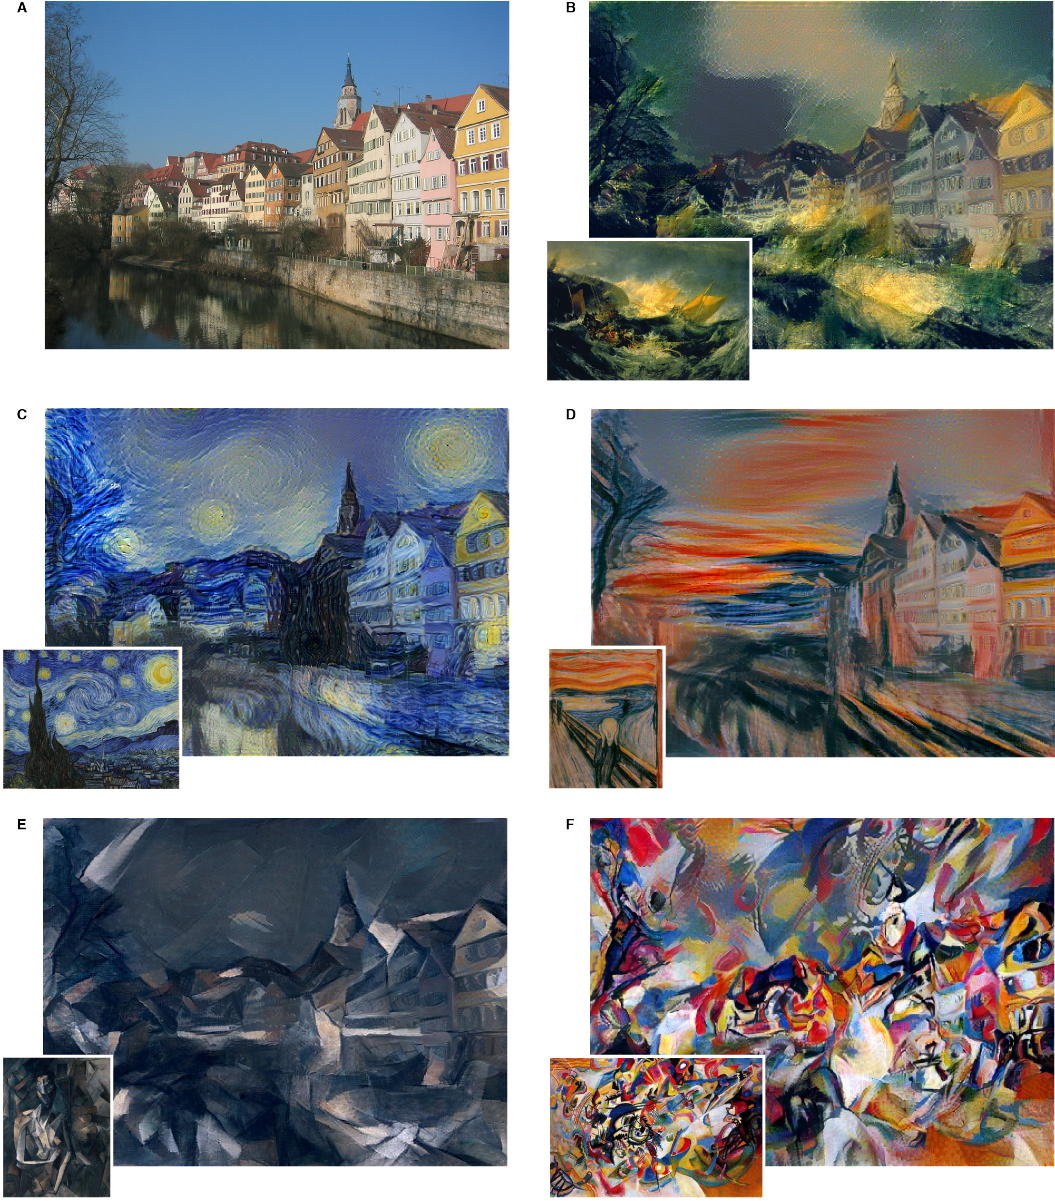
\includegraphics[width=\textwidth]{gfx/neural-style-examples}
  \caption{
    Images synthesized using the neural style algorithm \cite{Gatys2015B}.
    In \textbf{A}, the original photograph, depicting the Neckarfront in T\"ubingen, Germany, (shot by Andreas Praefcke).
    The style is applied from different artworks, shown in the bottom left corner of each panel.
    \textbf{B} \emph{The Shipwreck of the Minotaur} by J.M.W. Turner, 1805.
    \textbf{C} \emph{The Starry Night} by Vincent van Gogh, 1889.
    \textbf{D} \emph{Der Schrei} by Edvard Munch, 1893.
    \textbf{E} \emph{Femme nue assise} by Pablo Picasso, 1910.
    \textbf{F} \emph{Composition VII} by Wassily Kandinsky, 1913.
  }
  \label{sub:system:examples}
\end{figure}

In these examples we observe the style from several artworks is transferred to an original photograph.
The content of the photograph, its global arrangement, is effectively preserved while the style of the artworks, color, patterns, and local structures, is blended.
Unlike other attempts in style transfer, \todo{Check later}{as we have seen before}, neural style uses the feature space from a convolutional neural network trained in object recognition.


% ------------------------------------------------------------------------------

\section{Method}
\label{sec:system:method}

Neural style, simply put, takes two image sources: a photograph and an artwork, extracts the content from one and the style from the other, and generates a new image that matches both simultaneously.
The whole algorithm relies on a CNN already trained in object recognition to extract content and style from features found in source images.

\todo[inline]{Consider moving/connecting VGG-Network details to previous chapter}

\citeauthor{Gatys2015B}'s particular implementation uses VGG-Network \cite{Simonyan2014}, a CNN already trained in object recognition.
VGG-Network was designed and trained by the Visual Geometry Group at the University of Oxford with the goal of evaluating the performance of networks with increasing depth and it managed to score top results in ImageNet Challenge 2014.
The network achieved best results in between 16 and 19 weight layers with an architecture of convolutional filters with a very small receptive field (${3}\times{3}$, the smallest that can capture the notion of left/right, up/down and center) stride set to 1 pixel, and zero-padding to 1 pixel as well to preserve the original resolution of the input after the convolution.
Subsampling is performed by 5 max-pooling layers, inserted after some of the convolutional layers, over a ${2}\times{2}$ pixel window with stride set to 2 pixels so that the filter does not have overlapping input.

The VGG-Network implementation in Caffe framework is available under Creative Commons Attribution License \cite{Simonyan2014web}.
Among the 19-layer VGG-Network, neural style uses all 16 convolutional and 5 pooling layers, but none of the fully-connected layers, since classification is not required.
Max-pooling is replaced by average pooling because it produces a smoother gradient flow \cite{Boureau2010} and it results in cleaner synthesized images.
Lastly, for practical reasons, the weights in the networks are rescaled such that the mean activation of each filter over images and positions is equal to one.
Rescaling weights in this manner is always possible without affecting the output of the CNN when the activation functions are normalized with a ReLU layer like is the case in VGG-Network.

In a bit more detail, these are the algorithm's main stages: 1) both images get processed by the VGG-Network to produce their feature spaces, 2) content and style are extracted from those, and finally 3) a new image that matches them both is generated through backpropagation.

We will focus next on what we mean by content and style exactly and then how VGG-Network can synthesize new images that match content or style representations from a source image.
At the end, it will be obvious how it is possible to transfer the style using the neural style algorithm.


\subsection{Feature Representations}
\label{sub:system:method:representations}

Content and style of an image in neural style is characterized making use of the feature space produced by the VGG-Network.
If we remember the introduction on CNNs discussed in \autoref{sec:theory:convnets}, an original input gets transformed by filters defined in each layer as it moves across the network during the feed-forward phase.
To be more precise, a layer produces as many feature maps as filters it defines, each one of them highlighting different features of the input and represented by neural activations.
Spatially, we can imagine the output from a layer as a volume in which each slice is a feature map where neuron responses are arranged in 2D grids.
In image recognition tasks, each feature map is actually another image where pixels are active wherever the feature captured by the associated filter is present.

\paragraph{Content Representation}
We can also understand it the other way around, perceiving neural activations at a certain layer as an abstract representation of the original input image.
As a result of the VGG-Network having been trained in object recognition, its learned filters capture spatial information of the original input image, and thus, we can talk of the neural activations from a CNN layer as the content representation.
Formalizing it for an input image $\vec{x}$, let $l$ be a layer that applies $N_l$ different filters and produces $N_l$ feature maps of size $M_l$, where size is defined by the resolution ${height}\times{width}$ of the feature maps.
Vectorizing the feature maps, the total neural response at layer $l$ can be stored in a 2D matrix $F^l \in \mathbb{R}^{{N_l}\times{M_l}}$ where $F^l_{ij}$ is the feature activation for the $i^{th}$ filter at neuron $j$.

\begin{equation}
  F^l =
  \underbrace{
    \begin{bmatrix}
      F^l_{11}   & F^l_{12}   & \dots  & F^l_{1M_l} \\
      F^l_{21}   & F^l_{22}   & \dots  & F^l_{2M_l} \\
      \vdots     & \vdots     & \ddots & \vdots   \\
      F^l_{N_l1} & F^l_{N_l2} & \dots  & F^l_{N_lM_l}
    \end{bmatrix}
  }_{\text{vectorized feature maps}}
  \begin{matrix*}[l]
    \leftarrow & \text{filter } 1 \\
    \leftarrow & \text{filter } 2 \\
    \vdots                     \\
    \leftarrow & \text{filter } N_l
  \end{matrix*}
\end{equation}

\paragraph{Style Representation}
VGG-Network, as stated before, was not trained in any kind of style recognition task, so it is clear there is no style representation of any sort directly available in the network.
Nonetheless, \citeauthor{Gatys2015A} described in a previous work \cite{Gatys2015A} a method to build a style representation on top of the content representations without having to modify the network.
While the concept of content representation is somewhat intuitive to comprehend, style representation will require us to take a short detour to explain what we mean with style and what we expect its representation to be.

\citeauthor{Gatys2015A} approach style as a texture.
Texture synthesis tries to extract a texture model from an initial example so that arbitrary new samples of textures can be produced from it.
The quality of the model is normally evaluated by how hard it is for human inspection to distinguish between original and generated.
A texture model cannot be described by its exact pixel representation, rather a texture model must be uniquely described by statistical measurements, referred to as summary statistics, as was originally proposed by \citet{Julesz1962}.
We can understand this better by looking at \autoref{sub:system:method:style-reconstruction:texture}, showing a randomly generated image with 4 levels of brightness where a different texture has been applied on either half.
On the one hand, it illustrates how textures are independent of exact pixel representation as the randomly generated grid does not affect our ability to distinguish both textures.
On the other hand, it proves summary statistics are a better metric to distinguish one pattern from another.
This means that, within a texture model, any image that presents the same summary statistics as another, although having a different exact representation, can be considered the same texture.

\begin{figure}[htb]
  \begin{subfigure}[b]{0.5\textwidth}
    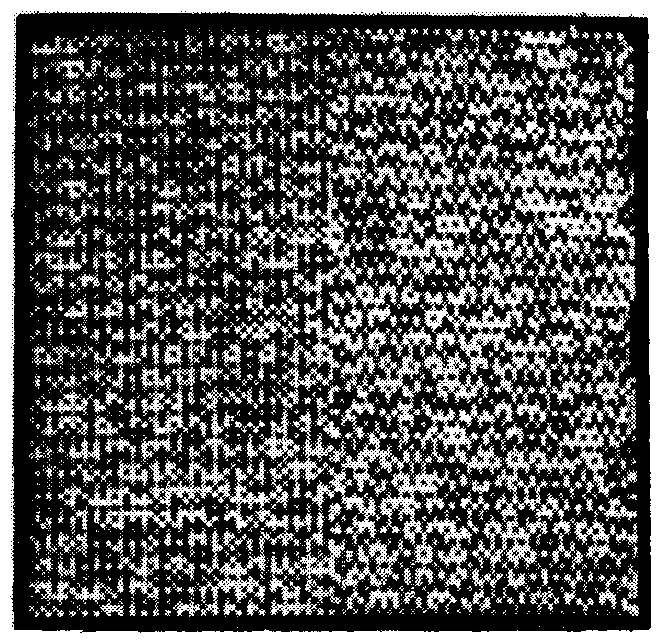
\includegraphics[width=\textwidth]{gfx/texture-1}
    \caption{Two-texture image}
    \label{sub:system:method:style-reconstruction:texture-1}
  \end{subfigure}
  \hfill
  \begin{subfigure}[b]{0.5\textwidth}
    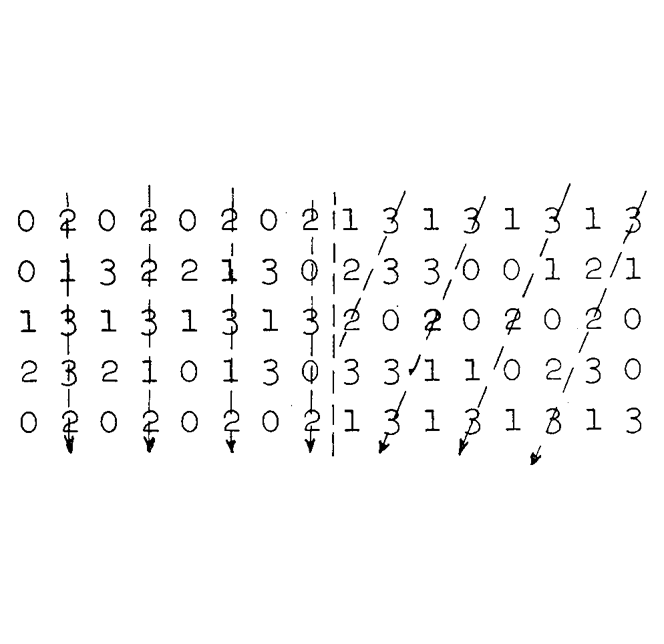
\includegraphics[width=\textwidth]{gfx/texture-2}
    \caption{Texture pattern generation}
    \label{sub:system:method:style-reconstruction:texture-2}
  \end{subfigure}
  \caption{Pattern discrimination \cite{Julesz1962}.
    On the left (a), an image with two different textures clearly visible.
    On the right (b), the pattern used to generate different textures on both halves of the image.
    Numbers represent the level of brightness and those outside of the arrows are randomly distributed.
    While no two regions on either half of the image are the same (brightness random distribution), the underlying patterns existing on each half (arrows) make them clearly distinguishable.}
  \label{sub:system:method:style-reconstruction:texture}
\end{figure}

Texture synthesis was later inspired by human visual systems, using Gabor filters for edge detection, which proved to be very similar to the human visual system \cite{Heeger1995,Portilla2000} and statistical measurements in these cases were taken over Gabor filter responses rather than on image pixels.
Results presented by \citet{Portilla2000} are probably still the best produced to date \cite{Gatys2015A}, but the method required careful handcrafting summary statistics that would result in good texture models.
Because of this, \citeauthor{Gatys2015A} argued \citeauthor{Portilla2000}'s method fails to generalize the full extent of natural textures and proposed in \cite{Gatys2015A} a method that combines the use of summary statistics with the feature space of a CNN already trained in object recognition, which fully models the human visual system.

Picking up again the analogy between textures and style, the summary statistic of the texture model is what we refer to as the style representation.
Since textures models are per definition stationary, the style representation must discard the spatial information existing in feature maps while keeping the notion of patterns.
One way to achieve it is by calculating the correlations between features maps in a CNN layer.
We can, therefore, formalize the style representation of an image $\vec{x}$ as a set of per-layer feature correlations $\{G^1, G^2, \dots, G^L\}$, where per-layer feature correlations are stored in 2D Gram matrixes $G^l \in \mathbb{R}^{{N_l}\times{N_l}}$ \cite[Theorem~7.2.10]{Horn2012}:

\begin{equation}
  G^l =
  \begin{bmatrix}
    G^l_{11}   & G^l_{12}   & \dots  & G^l_{1N_l} \\
    G^l_{21}   & G^l_{22}   & \dots  & G^l_{2N_l} \\
    \vdots     & \vdots     & \ddots & \vdots   \\
    G^l_{N_l1} & G^l_{N_l2} & \dots  & G^l_{N_lN_l}
  \end{bmatrix}
\end{equation}

Being $G^l_{ij}$ the inner product between the vectorized feature maps $i$ and $j$ in layer $l$, representing their degree of correlation:

\begin{equation}
  G^l_{ij} =
  \begin{bmatrix}
    F^l_{i1} & \dots & F^l_{iM_l}
  \end{bmatrix}
  \begin{bmatrix}
    F^l_{j1} \\
    \vdots \\
    F^l_{jM_l}
  \end{bmatrix}
  = \sum_k F^l_{ik}F^l_{jk}
\end{equation}

Having defined content and style representations we can now move to discussing how they can be used to produce new images.
\citeauthor{Gatys2015B} refer to this process feature reconstruction.


\subsection{Feature Reconstruction}
\label{sub:system:method:reconstructions}

In neural style algorithm, feature reconstruction is the process of visualizing some feature representation of an original input image.
The visualization is, in fact, a new image $\vec{x}$ that must be generates so that either its content representation or its style representation matches that of the original input image.
We will talk about \emph{content reconstruction} when the new image $\vec{x}$ is generated so that matches the content representation and \emph{style reconstruction} when it does so with the style representation.
The strategy to generates the new image $\vec{x}$ is approaching the task as an optimization problem very much like backpropagation, as we will see next.

\paragraph{Content reconstruction}
Starting from a random white noise image $\vec{x}$, we want to transform it so that it becomes the image $\vec{x}$ whose content representation is the same as the original photograph $\vec{p}$ at a certain layer $l$.
It is then the difference between content representations of $\vec{x}$ and $\vec{p}$ what we need to minimize.
So, let $P^l$ and $F^l$ be the content representations of the original photograph $\vec{p}$ and the generated image $\vec{x}$, respectively, in layer $l$, we define the loss function to be minimized as the squared error between the two representations:

\begin{equation}
  \mathcal{L}_{content}(\vec{p}, \vec{x}, l) = \frac{1}{2} \sum_{i,j}(F^l_{ij}-P^l_{ij})^2
\end{equation}

With this loss function we want to ultimately modify the white noise image $\vec{x}$, which can be perceived as the content representation at the input layer $l = 0$, so we can say we want to find the partial derivative of the loss with respect to the content representation such as:

\begin{equation}
  \Delta \vec{x} =
  \frac{\partial \mathcal{L}_{c}}{\partial \vec{x}} =
  \frac{\partial \mathcal{L}_{c}}{\partial F^0}
\end{equation}

Which generalized for any layer $l$ with the chain rule can be analytically calculated for every neuron as:

\begin{equation}
  \mathcal{L}^l_{ij} =
  \frac{\partial \mathcal{L}_{c}}{\partial F^l_{ij}} =
  \begin{cases}
    (F^l - P^l)_{ij} & \text{if } F^l_{ij} > 0 \\
    0                & \text{if } F^l_{ij} < 0
  \end{cases}
\end{equation}

We can then apply standard error backpropagation \cite{Orr2008} as depicted in \autoref{fig:system:method:feature-reconstruction} to calculate the gradients for each pixel of the white noise image $\vec{x}$.
With them, we can adjust $\vec{x}$ until its content representation matches that of the photograph $\vec{p}$ at layer $l$.

\begin{figure}[htb]
  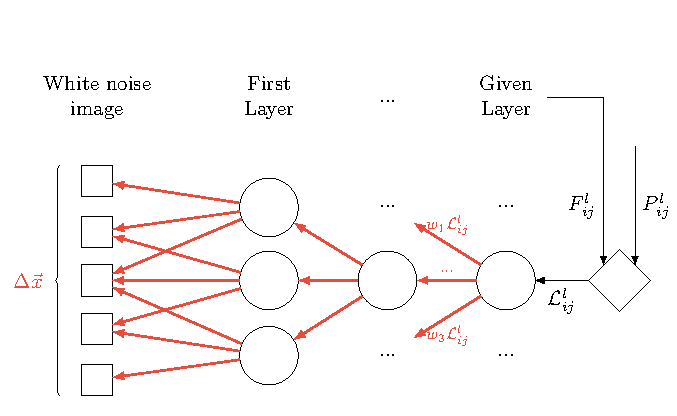
\includegraphics[width=\textwidth]{tkz/feature-reconstruction}
  \caption{
    Content reconstruction with standard backpropagation.
    The content loss $\mathcal{L}^l_c$ is numerically calculated for each neuron in a given layer $l$ from the content representation $F^l$ and $P^l$, resulting from the feed-forward pass of the white noise image $\vec{x}$ and the photograph $\vec{p}$ respectively.
    The calculated loss is backpropagated through the whole network until it reaches the first layer.
    The gradients $\Delta \vec{x}$ for adjusting the white noise $\vec{x}$ are calculated in the same way as if the input layer is a CNN layer.
  }
  \label{fig:system:method:feature-reconstruction}
\end{figure}

\paragraph{Style reconstruction}
Similarly, starting from a random white noise image $\vec{x}$, we will transform it to that it matches the style representation of an original artwork $\vec{a}$ in a number of CNN layers.
So, let $A^l$ and $G^l$ be the style representations of the original artwork $\vec{a}$ and the generated image $\vec{x}$, respectively, in layer $l$, we define the error as the mean-squared distance between the two representations:

\begin{equation}
  E_l =
  \frac{1}{4 N^2_l M^2_L} \sum_{i,j} (G^l_{ij} - A^l_{ij})^2
\end{equation}

Note this is not the loss function, since, unlike content representation, style representation is defined by the feature correlations $\{G^1, G^2, \dots, G^L\}$ in a number of layers.
Thus, we define the loss function to be minimized in style reconstruction as:

\begin{equation}
  \mathcal{L}_{style}(\vec{a}, \vec{x}) =
  \sum_{l \in L} w_l E_l
\end{equation}

Where $w_l$ are relative weights representing the contribution of each layer to the total loss $\mathcal{L}_{s}$.
Now, to obtain the gradients that will correct the white noise image $\vec{x}$ we must find the partial derivative of the loss function with respect to it.

\begin{equation}
  \Delta \vec{x} =
  \frac{\partial \mathcal{L}_{s}}{\partial \vec{x}}
\end{equation}

We can express the total loss in terms of the per-layer error as:

\begin{equation}
  \Delta \vec{x} =
  \frac{\partial \mathcal{L}_{s}}{\partial \vec{x}} =
  \frac{\partial \mathcal{L}_{s}(E_1, E_2, \dots, E_L)}{\partial \vec{x}}
\end{equation}

Which, applying the chain rule as described in \cite[Eq. 3.23]{Hairer2008}, can be rewritten as:

\begin{equation}
  \Delta \vec{x} =
  \sum_{l \in L} \Bigg(\frac{\partial \mathcal{L}_s}{\partial E_l} \frac{\partial E_l}{\partial \vec{x}}\Bigg) =
  \sum_{l \in L} \Bigg(w_l \frac{\partial E_l}{\partial \vec{x}}\Bigg)
\end{equation}

At this point, the only thing missing is calculating the derivative of the layer error $E^l$ with respect to the white noise image $\vec{x}$.
Finally, assuming $\vec{x}$ is the content representation $F^l$ in layer $l = 0$, we can generalize it for any layer $l$ by applying again the chain rule, which calculated for every neuron is expressed as:

\begin{equation}
  \frac{\partial E_l}{\partial F^l_{ij}} =
  \begin{cases}
    \frac{1}{N^2_l M^2_L} ((F^l)^T (G^l - A^l))_{ij} & \text{if } F^l_{ij} > 0 \\
    0                                                & \text{if } F^l_{ij} < 0
  \end{cases}
\end{equation}

Like in content representation, the gradients $\Delta \vec{x}$ can be obtained with standard error backpropagation to adjust the white noise $\vec{x}$ until its style representation matches that of $\vec{a}$ for the selected set of feature correlations $\{G^1, G^2, \dots, G^L\}$.

The results of separately reconstructing content and style can be seen in \autoref{sub:system:method:reconstructions}.
In content reconstruction, at the bottom, while visualizations generated from lower layers (a, b, c) preserve pixel fidelity compared with the input image, those generated from higher layers (d, e) lose pixel fidelity, since due to subsampling effects there is not enough information in the layer to exactly reconstruct the input image.
High-level content information is preserved in all cases, nonetheless, because the reconstruction process makes the neural activations produced by the input image and the generated one match, proof that feature maps in VGG-Network, trained in object recognition, precisely capture spatial information.
This is useful for the neural style algorithm to produce less hyperrealistic results when combining a photograph with an artwork.
In style reconstructions, at the top, visualizations have been generated with increasingly larger subsets of layers.
We observe how the texture transitions from colored noise (a), to just a cloud of colors (b), to clearer strokes (c, d), to bigger structures from the original artwork (d).
This is a consequence of the larger perceptive field of the filters in higher layers being able to capture bigger patterns that ultimately get transferred to the generated texture.
Being able to parametrize the texture is useful in the neural style algorithm to tweak how much detail of the style should be transferred, like in this example, where it should be small if we just want to transfer the characteristic style of strokes of Vincent van Gogh (b, c), or big if we also want shapes like the moon, clouds and the tower in \emph{The Starry Night}.

\begin{figure}[htb]
  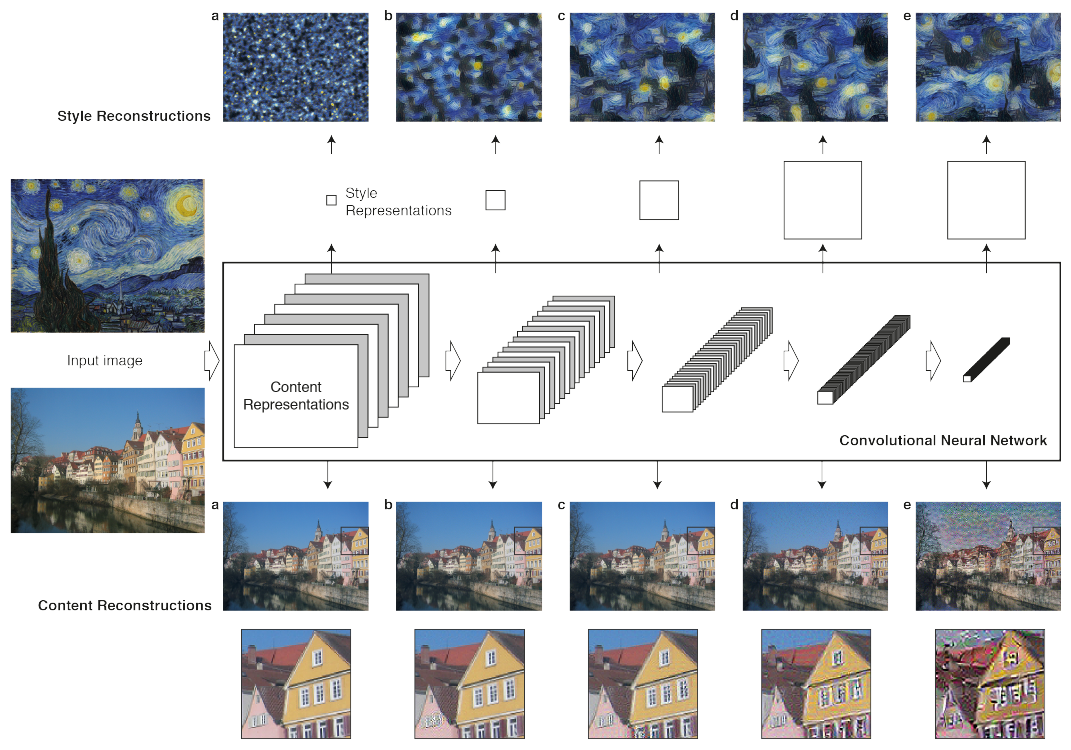
\includegraphics[width=\textwidth]{gfx/neural-style-cnn}
  \caption{
    Content and style reconstructions from an artwork and a photograph, respectively, using different feature maps from a CNN \cite{Gatys2015B}.
    As the input image gets processed by the CNN an increasing number of filter maps get produced in each layer.
    The totality of them for one layer are referred to in neural style as the content representation of the input image.
    At the bottom, content reconstructions of the photograph are generated at different stages of the VGG-Network from the following layers: ``conv1\_1'' (a), ``conv2\_1'' (b), ``conv3\_1'' (c), ``conv4\_1'' (d) and ``conv5\_1''.
    Style representations of an input image are built on top of content representations from a set of layers.
    At the top, style reconstructions of the artwork are generated using increasingly big subsets of layers: ``conv1\_1'' (a), ``conv1\_1'' and ``conv2\_1'' (b), ``conv1\_1'', ``conv2\_1'' and ``conv3\_1'' (c), ``conv1\_1'', ``conv2\_1'', ``conv3\_1'' and ``conv4\_1'' (d), ``conv1\_1'', ``conv2\_1'', ``conv3\_1'', ``conv4\_1'', and ``conv5\_1''.
    Including content representations from higher layers make the receptive field of style representations increase in size, and thus, the style reconstructions present larger local structures from the original artwork.
  }
  \label{sub:system:method:reconstructions}
\end{figure}


\subsection{Mixed Representation}
\label{sub:system:method:mixed-representation}

Having described how to separately reconstruct content and style from an original image it is straightforward to explain how the neural style algorithm is capable of simultaneously reconstructing both content and style from two different sources and producing the images in \autoref{sub:system:examples}.

Like in the previous cases, we want to find a new image $\vec{x}$ whose content representation and style representation matches at the same time the content representation of a photograph $\vec{p}$ in a given layer and the style representation of an artwork $\vec{a}$ in a set of layers.
Starting from a white noise image $\vec{x}$ the algorithm will simply need to minimize the following combined loss function:

\begin{equation}
  \mathcal{L}_{total}(\vec{p}, \vec{a}, \vec{x}) =
    \alpha \mathcal{L}_{content}(\vec{p}, \vec{x}) +
    \beta \mathcal{L}_{style}(\vec{a}, \vec{x})
\end{equation}

Where $\alpha/\beta$ is the ratio of emphasis of content over style, since content and style cannot be completely disentangled and a trade-off must be manually adjusted for each pair of source images.
The gradients $\Delta \vec{x}$, as before, are calculated with standard error propagation and are used to adjust the white noise image $\vec{x}$ until it reaches a compelling result.
The optimization process is one of huge dimensionality, taking into account the 144 million parameters in VGG-19 \cite{Simonyan2014}, and the unconstrained resolution of source images, and so \citeauthor{Gatys2015A} propose L-BFGS \cite{Zhu1994} as a suitable gradient optimization strategy.


% ------------------------------------------------------------------------------

\section{Results}
\label{sec:system:results}

\todo[inline]{Use my own results if enough time}

\citeauthor{Gatys2015B} presented in \cite{Gatys2015B} a series of results to showcase how each different hyperparameter affect the outcome of the algorithm as they vary.
As hinted while explaining the reconstruction process, the hyperparameters taken into account are three: 1) the ratio of emphasis on content over style $\alpha / \beta$, 2) the relative weights given to the CNN layers for style representation $\vec{w}_L$, and 3) which CNN layer is used for content representation.

\autoref{fig:system:results} shows results of some variations arranged in a grid where columns show variation in emphasis on content over style and rows variation of relative weights for style representation, having content representation fixed to CNN layer ``conv4\_2'' of the VGG-Network.
Although the style reconstruction method allows for arbitrary relative weights, \citeauthor{Gatys2015B} fixed on a simpler approach only using increasingly higher CNN layers and giving them equal relative weights.
In such configuration, relative weights for active CNN layers is set to $w_l = 1/n$, being $n$ the number of active layers, and to $w_l = 0$ for the rest.
Active CNN layers for style reconstruction per row: A) only ``conv1\_1'' ($w_l = 1$), B) ``conv1\_1'' and ``conv2\_1'' ($w_l = 1/2$), C) ``conv1\_1'', ``conv2\_1'' and ``conv3\_1'' ($w_l = 1/3$), D) ``conv1\_1'', ``conv2\_1'', ``conv3\_1'' and ``conv4\_1'' ($w_l = 1/4$), and finally E) ``conv1\_1'', ``conv2\_1'', ``conv3\_1'', ``conv4\_1'', and ``conv5\_1'' ($w_l = 1/5$).

\begin{figure}[!tb]
  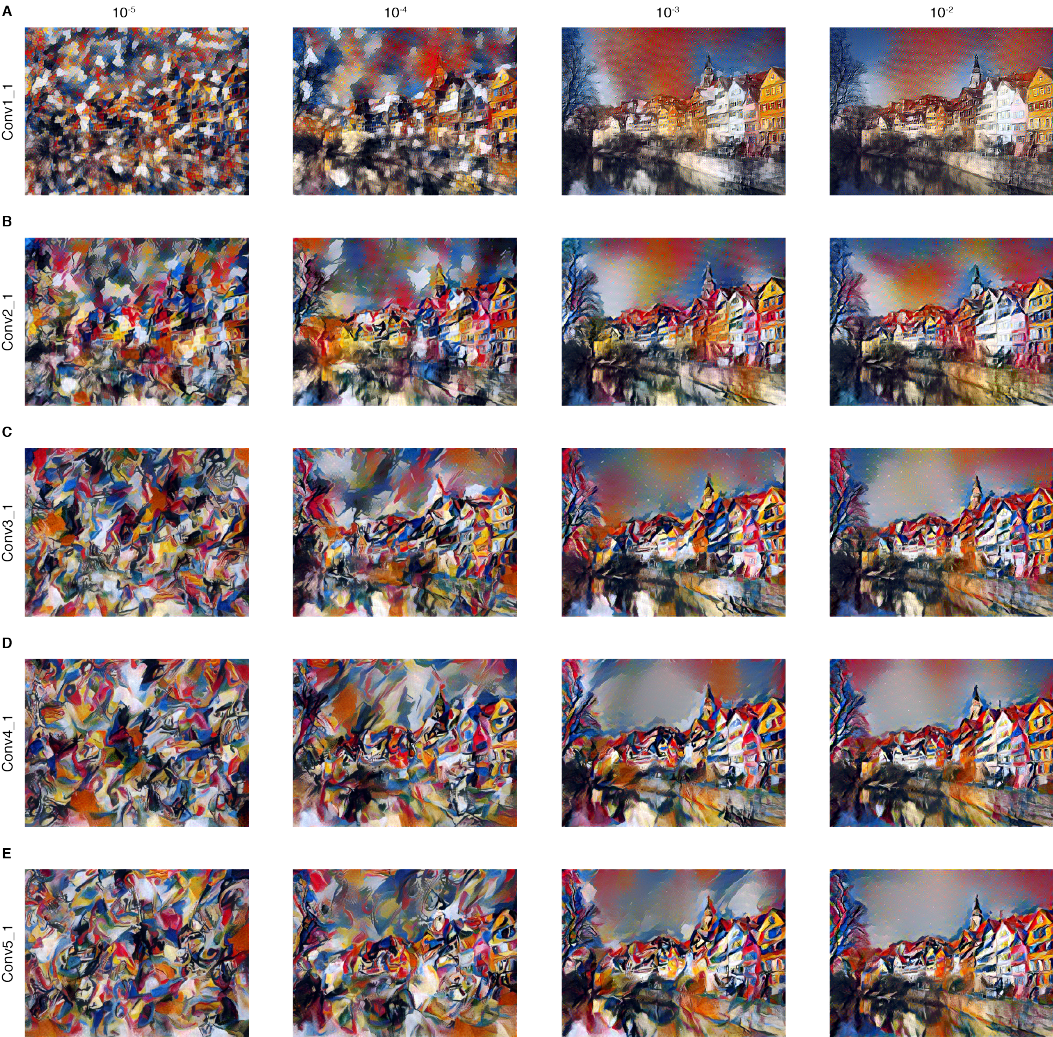
\includegraphics[width=\textwidth]{gfx/neural-style-results}
  \caption{
    Neural Style hyperparameter variation results of combining a photograph with the style of \emph{Composition VII} by Wassily Kandinsky.
    In the rows, from top to bottom, the increasing subset of CNN layers used for style representation, expressed with the higher layer used from VGG-Network (up to $conv\#\_1$).
    In the columns, from left to right, the increasing ratio $\alpha / \beta$ representing the emphasis on content over style.
    Including style features from higher layers of the network results in the style representation capturing bigger and more complex from the original artwork.
    Higher emphasis on content over style results in the synthesized image preserving more features of the original photograph.
  }
  \label{fig:system:results}
\end{figure}

Variations in emphasis on content over style show how increasing this ratio results on the features of the original photograph being preserved more faithfully.
If we look at \autoref{fig:system:results}~(A1), with a ratio of $10^{-5}$, very little is kept from the spatial information of the photograph and only some blue puffs representing the sky can be seen in the top region.
In \autoref{fig:system:results}~(A2), with a ratio of $10^{-4}$, the overall spatial arrangement of the photograph is already discernible, but, other than the closest building, the exact elements of the rest of the photograph are hard to tell.
Already in \autoref{fig:system:results}~(A3), with a ratio of $10^{-3}$, the buildings, river and tree are finally appreciable.
The exact spatial information remaining at the end is, however, dependent as well on the particular style representation chosen.

Now focusing on how the different style representations affect the outcome, we can see that including higher CNN layers makes the patterns increase in size and complexity.
The style representation captured ranges from showing little more than color puffs in \autoref{fig:system:results}~(A1), to similar shapes as seen in the original artwork in \autoref{fig:system:results}~(A5).
This makes sense if we think of CNNs trained in object recognition work.
Lower layers have small receptive fields and filters apply transformations that simply capture edges, corners or orientations.
On the other hand, higher layers have larger receptive fields due to subsampling and filters capture increasingly complex patterns such as shapes, text, or faces.

While Neural Style displays astounding capabilities for separation and mixing of style and content, compelling artistic results seem to be restricted to a particular region of hyperparameter values.
This region is not stationary as it varies from case to case depending on the photograph and artwork chosen and requiring careful fine-tuning of pixel fidelity (the chosen CNN layer for content representation), spatial information (the content-style ratio), and style representation complexity (the chosen CNN layers for style representation).


% ------------------------------------------------------------------------------

\section{Conclusion}
\label{sec:system:conclusion}

For the same reason \citeauthor{Gatys2015A} argues in \cite{Gatys2015A} about \citet{Portilla2000}'s approach not grasping the whole scope of natural textures which seems to have been solved I argue requiring human intervention for finding a set of hyperparameters in Neural Style that produce human compelling artistic composition is letting me think we are still far from understanding what describes art.

Neural Style astonishing results have caused quite a stir since they were presented in 2015.
In the next chapter, we will see how it has impacted the machine learning research community with derived work and promising further applications.

\todo[inline]{Complete discussion so that it connects with next chapter}

% All in all it is truly fascinating that a neural system, which is trained to perform one of the core computational tasks of biological vision, automatically learns image representations that allow the separation of image content from style. The explanation could be that when learning object recognition, the network has to become invariant to all image variation that preserves object identity. Representations that factorise the variation in the content of an image and the variation in its appearance would be extremely practical for this task. Thus, our ability to abstract content from style and therefore our ability to create and enjoy art might be primarily a preeminent signature of the powerful inference capabilities of our visual system.

% To understand our texture features better in the context of the original object recognition task of the network, we evaluated how well object identity can be linearly decoded from the texture features in different layers of the network. For each layer we computed the Gram-matrix representation of each image in the ImageNet training set [23] and trained a linear soft-max classifier to predict object identity. As we were not interested in optimising prediction performance, we did not use any data
% augmentation and trained and tested only on the 224×224 centre crop of the images. We computed the accuracy of these linear classifiers on the ImageNet validation set and compared them to the
% performance of the original VGG-19 network also evaluated on the 224 × 224 centre crops of the validation images.

% The analysis suggests that our texture representation continuously disentangles object identity in- formation (Fig. 4). Object identity can be decoded increasingly well over the layers. In fact, linear decoding from the final pooling layer performs almost as well as the original network, suggesting that our texture representation preserves almost all high-level information. At first sight this might appear surprising since the texture representation does not necessarily preserve the global structure of objects in non-texture images (Fig. 2, last column). However, we believe that this “inconsistency” is in fact to be expected and might provide an insight into how CNNs encode object identity. The convolutional representations in the network are shift-equivariant and the network’s task (object recognition) is agnostic to spatial information, thus we expect that object information can be read out independently from the spatial information in the feature maps. We show that this is indeed the case: a linear classifier on the Gram matrix of layer ‘pool5’ comes close to the performance of the full network (87.7% vs. 88.6% top 5 accuracy, Fig. 4)

% We envision that this will be useful for a wide range of experimen- tal studies concerning visual perception ranging from psychophysics over functional imaging to even electrophysiological neural recordings
% The style representations simply compute the correlations between different types of neurons in the network. Extracting correlations between neurons is a bio- logically plausible computation that is, for example, implemented by so-called complex cells in the primary visual system (V1)
% \cite{Adelson1985}
	% INCLUDE: system
% !TEX root = ../thesis-example.tex
%
\chapter{Concepts: This text is here to test a very long title, to simulate the line break behavior, to show that an extremely long tilte also works}
\label{sec:concepts}

\cleanchapterquote{Users do not care about what is inside the box, as long as the box does what they need done.}{Jef Raskin}{about Human Computer Interfaces}

\Blindtext[2][1]

\section{Concepts Section 1}
\label{sec:concepts:sec1}

\Blindtext[2][2]

\section{Concepts Section 2}
\label{sec:concepts:sec2}

\Blindtext[3][2]

\section{Concepts Section 3}
\label{sec:concepts:sec3}

\Blindtext[4][2]

\section{Conclusion}
\label{sec:concepts:conclusion}

\Blindtext[2][1]
 % INCLUDE: concepts
% !TEX root = ../thesis.tex

\chapter{Conclusion}
\label{chap:conclusion}

\cleanchapterquote{“Knowledge is just opinion that you trust enough to act upon.}{Orson Scott Card}{(Children of the Mind)}


% ------------------------------------------------------------------------------

In Chapter~\ref{chap:theory} we saw multi-layer feedforward neural networks are universal approximators.
A sufficiently big fully-connected network could, theoretically, solve arbitrarily complex problems.
However, limited computational resources and training datasets make them unpractical for real-world tasks.
Deep neural networks are used instead, as they learn increasingly abstract notions instead of raw inputs and require much fewer learnable parameters.
Traditionally, pattern recognition algorithms required domain features to be carefully modeled by experts with knowledge on the field, but Deep Learning allows us to train neural networks to carry out feature engineering automatically for us.

In Chapter~\ref{chap:context} we reviewed how the feature extraction capabilities of deep neural networks consistently granted them the top positions in object recognition challenges.
It is remarkable how well we understand how to make neural networks work for object recognition, as they now rival human performance in many aspects, compared to how little we know about how they reason once they are trained.
To help understanding this, recently-developed techniques try to visualize internal representations of deep neural networks and have produced very intriguing images with with potential artistic implications.

In Chapter~\ref{chap:system} we presented the Neural Style algorithm and how it managed to solve a long-standing problem in artistic rendering: the separation of style and content.
Whereas the algorithm can produce visually compelling compositions of style and content from two different source images, it requires fine-tuning on a per-case basis.
This make us believe Neural Style fails to grasp the notion of ``aesthetics'', which is another unsolved problem in artistic rendering, often studied in \emph{algorithmic aesthetics}.

In Chapter~\ref{chap:applications} we surveyed a number of methods for improved style transfer and several other image transformation tasks that also rely on extracting visually perceptive features.
They all presenting superior performance than the state of the art in their respective field.

The separation of style and content had been a very difficult problem to solve because it depends on human non-objective perception of what is style and what is content in an artwork.
Formulating notions of ``aesthetics'' is a similarly complex problem, since we cannot formally define it and totally builds upon human perception.

Capturing subjective opinions is being currently researched.
At the time of writing this thesis, the Beauty.AI's First International Beauty Contest Judged by an Artificial Intelligence Jury \cite{YouthLaboratories} has taken place already.
Their promoters, supported by Nvidia and Microsoft among others, aim for teaching machines estimate human attractiveness by looking at the human face, relying for this on human biased perception.

In the light of the increasing interest in distilling inherently subjective features that are impractically to model formally, we find the study of aesthetics a relevant matter with practical applications.
Therefore, we believe the aesthetics of images could be similarly distilled and used for further improving artistic rendering techniques.


% ------------------------------------------------------------------------------

\section{Future Work}
\label{sec:conclusion:future}

We propose further work on building an aesthetics-driven deep neural network for style transfer.
The system would consist of two sub-networks: one for image transformations, and another for quality estimation.
The image transformation network, once trained, would produce perceptually compelling images.
For training it, an aesthetic estimation network would rate the perceptual quality of the generated images and this would be used as the loss function.

The first challenge is finding how to quantify the perceptual quality of an image.
That is, to model an inherently human subjective notion.
For that we propose a convolutional neural network (CNN) that should be trained for estimating aesthetics based on human opinion.
The network could be either trained from scratch or from one pre-trained for object recognition, applying transfer learning techniques \cite{Pan2010}, which basically allows the network to adjust to a slightly different task or domain.

In order to train the aesthetics estimation network we must have a sufficiently large and diverse training dataset of image-rating pairs.
We imagine a crowdsourcing platform with which to collect ratings from humans on artistic compositions.
People would be presented with two artistic images and they should decide which two of them appeal most to them.
This is currently being done similarly in DeepArt.io's for the artistic Turing test (\url{https://turing.deepart.io/}).

The artistic images people would be rating could be composed of images from three sources: 1) a repository of classical paintings, 2) user-submitted style transfer creations, and 3) randomly-generated style transfer creations.
This last source would be generated from the repository of classical paintings, some repository of photographs, and randomly chosen style transfer hyperparameters.
Including them is of particular interesting since it will result in a more diverse, less biased artistic creations, and once ratings are collected, therefore, in a more representative training dataset for the aesthetic estimation network.

Important considerations to be taken when deploying the crowdsourcing initiative would be: acquiring a sufficiently large initial repository of images to rate, incentives to invite people to contribute, user interaction design to keep the contribution process simple, and, finally, potential partnerships with industry for having access to computation facilities in which to run the initiative.

The second challenge, once the aesthetic estimation network had been trained, is designing and training the image transformation network.
We have identified three plausible directions thus far.

Our first intuition is using a CNN whose very last layer is the Neural Style algorithm, as is.
The image transformation network in this case would learn how the Neural Style hyperparameters must be adjusted to produce a perceptually compelling composition given a pair of source images.

Likewise, our second approach is having the Neural Style hyperparameters fixed to some relatively good values.
In this case, the image transformation network would instead learn how to correct the source images so that when processed by Neural Style the result would be appealing.

We anticipate two main problems with the previous approaches.
First, Neural Style is computationally expensive, as it requires of a backpropagation pass to produce the images, and relying on it would terribly slow down the learning process.
And second, we suspect reusing Neural Style as a black box layer would limit the meaning of the internal representations.

To circumvent this, and inspired by \cite{Johnson2016}'s approach, we would completely disregard Neural Style in the image transformation network.
The network would learn how to maximize the perceived quality of the composition for a fixed style and a given photograph in a simple feedforward pass.
The question is still open to see if the network could learn how to apply general style transfer given two images.
We conjecture, however, that, by using the aesthetics estimation network as part of the loss function, it can be possible.

We are certain, such a system will not only pose a versatile tool for artistic rendering, it will also be of great relevance to the advance in neuroscience.
Giving researchers a new way to look into how the creative process occurs in the human brain and what are the patterns in nature that elicit the notion of beauty in our minds.

\begin{figure}[!b]
  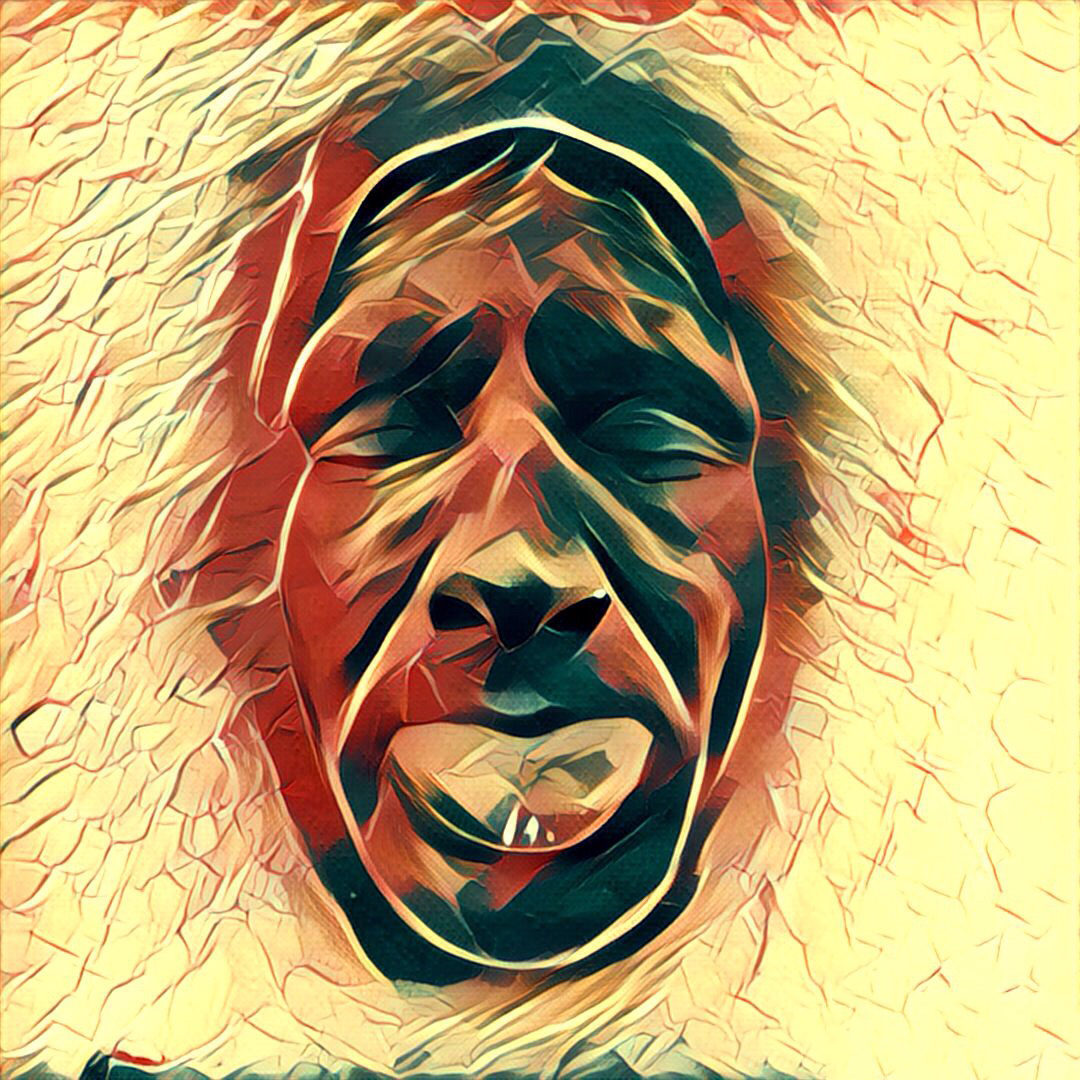
\includegraphics[width=\textwidth]{gfx/prisma}
\end{figure}
 % INCLUDE: conclusion
\cleardoublepage

% --------------------------
% Back matter
% --------------------------
{%
\setstretch{1.1}
\renewcommand{\bibfont}{\normalfont\small}
\setlength{\biblabelsep}{0pt}
\setlength{\bibitemsep}{0.5\baselineskip plus 0.5\baselineskip}
\printbibliography[nottype=online]
\printbibliography[heading=subbibliography,title={Webseiten},type=online,prefixnumbers={@}]
}
\cleardoublepage

\listoffigures
\cleardoublepage

\listoftables
\cleardoublepage

% !TEX root = ../thesis.tex
%
\pagestyle{empty}
\hfill
\vfill
\pdfbookmark[0]{Colophon}{Colophon}
\section*{Colophon}

This thesis was typeset with \LaTeXe.
It uses the \textit{Clean Thesis} style developed by Ricardo Langner.
The design of the \textit{Clean Thesis} style is inspired by user guide documents from Apple Inc.

Download the \textit{Clean Thesis} style at \url{http://cleanthesis.der-ric.de/}.

\cleardoublepage

% !TEX root = ../thesis.tex

\pdfbookmark[0]{Declaration}{Declaration}
\chapter*{Declaration}
\thispagestyle{empty}

I declare that I have completed my work solely and only with the help of the references mentioned above.

\bigskip
\noindent\textit{\thesisUniversityCity, \thesisDate}

\smallskip
\begin{flushright}
	\begin{minipage}{5cm}
		\rule{\textwidth}{1pt}
		\centering\thesisName
	\end{minipage}
\end{flushright}

\clearpage
\newpage
\mbox{}

% **************************************************
% End of Document CONTENT
% **************************************************
\end{document}
